% questions.tex —— 1977 年·浙江卷 · 题目内容片段（无答案）
% 由 tools/generate_projects.py 依来源总账自 1977/1977_数学真题_浙江_试题.md 生成，勿手改（改源 MD 后重跑）


\gkpart{数学试题解（浙江卷）}

\begin{gktip}
\textbf{来源说明}：本题面依据固定源 PDF《浙江1977年高考数学试题解》第 1—4 页逐题转录。源卷是题面与解答连续排印的《试题解》材料（每题题面后紧跟「解：」或「证明：」），解答不随题面转录，由本库对照复算后写入配套解析；原卷第 1—3 页底部带书籍页码 61—63，第 4 页无页码，本文按 PDF 页序记录。原卷大题以汉数字「一、二、……、七」编号、大题内小项以阿拉伯数字编号，本库按规范将大题重排为阿拉伯数字 1—7、小项重排为（1）（2）（3），未增删题干。正式题各题标注（本题 X 分），合计 100 分；末尾「参考题（不计分，可以不做）」两题不计入题量。
\end{gktip}

\par\medskip

\begin{question}
\gkti{1}计算：

（1） $\sqrt[6]{8^5}\div\sqrt{8}\times\sqrt[3]{8}\div\left(\dfrac18\right)^0$（本题 5 分）。

（2） $\dfrac{\lg 4+\lg 25-\lg 10}{\lg\sqrt{1000}}$（本题 5 分）。

（3） $\dfrac{1}{100\times101}+\dfrac{1}{101\times102}+\dfrac{1}{102\times103}+\cdots+\dfrac{1}{149\times150}$（本题 5 分）。

\Needspace{0.4\textheight}
\end{question}
\begin{question}
\gkti{2}

（1） 已知 $\operatorname{tg}\alpha=\sqrt2$，求 $\dfrac{\cos\alpha+\sin\alpha}{\cos\alpha-\sin\alpha}$ 的值（本题 5 分）。

（2） 求 $\sin^262^\circ+\operatorname{tg}54^\circ\cdot\operatorname{tg}45^\circ\cdot\operatorname{tg}36^\circ+\sin^228^\circ$ 的值（本题 5 分）。

（3） 某生产队要建一个贮粮用的“土圆仓”，如果土圆仓下部圆柱和上部圆锥的底面半径都是 1.5 米，高分别是 3 米和 0.6 米，计算它的容积（$\pi\approx3.14$，精确到 0.1 立方米）（本题 8 分）。

\begin{gktip}
原源 PDF 第 1 页右下附有土圆仓（下部圆柱、上部圆锥）示意图；LaTeX 版按源图重绘。
\end{gktip}
\nopagebreak[4]
\begin{center}% 1977 年浙江卷第 2(3) 题：贮粮“土圆仓”，下部圆柱、上部圆锥，
% 轴虚线自锥顶贯穿到底面圆心，标注圆锥高 0.6 米、圆柱高 3 米、底面半径 r=1.5 米（按源卷第 1 页布局）
\begin{tikzpicture}[scale=0.9]
  % 圆柱轮廓
  \draw[thick] (-1.6,0)--(-1.6,3);
  \draw[thick] (1.6,0)--(1.6,3);
  % 底面椭圆：后半虚线、前半实线
  \draw[dashed] (1.6,0) arc (0:180:1.6 and 0.42);
  \draw[thick] (1.6,0) arc (0:-180:1.6 and 0.42);
  % 顶面椭圆（即圆锥底面）：后半虚线、前半实线
  \draw[dashed] (1.6,3) arc (0:180:1.6 and 0.42);
  \draw[thick] (1.6,3) arc (0:-180:1.6 and 0.42);
  % 圆锥两条母线
  \draw[thick] (-1.6,3)--(0,4.15)--(1.6,3);
  % 轴线与半径（虚线）
  \draw[dashed] (0,4.15)--(0,0);
  \draw[dashed] (0,3)--(1.6,3);
  \draw[dashed] (0,0)--(1.6,0);
  % 标注
  \node[rotate=90] at (-0.34,3.6) {$0.6$ 米};
  \node[rotate=90] at (-0.34,1.5) {$3$ 米};
  \node at (0.78,-0.4) {$r=1.5$ 米};
\end{tikzpicture}
\end{center}
\nopagebreak[4]
\end{question}
\begin{question}
\gkti{3}\textbf{（15 分）} 求平行直线 $3x+2y-3=0$ 和 $3x+2y+2=0$ 之间的距离。

\end{question}
\begin{question}
\gkti{4}\textbf{（15 分）} 已知 $\alpha$ 和 $\beta$ 是三角形的两个内角，并且 $\alpha$ 是锐角，而 $\cos\alpha=\dfrac35$，$\sin\beta=\dfrac5{13}$，求 $\sin(\alpha+\beta)$ 的值。

\end{question}
\begin{question}
\gkti{5}\textbf{（15 分）} 解不等式：$\log_5(x^2-2x-15)<\log_5(x+13)$。

\Needspace{0.4\textheight}
\end{question}
\begin{question}
\gkti{6}\textbf{（10 分）} 点 $O$ 为 $\triangle ABC$ 内任意一点，连接 $AO$ 并延长交 $BC$ 于点 $D$，连接 $BO$ 并延长交 $AC$ 于点 $E$，连接 $CO$ 并延长交 $AB$ 于点 $F$，则

\nopagebreak[4]
\[
\frac{OD}{AD}+\frac{OE}{BE}+\frac{OF}{CF}=1.
\]

\begin{gktip}
原源 PDF 第 3 页附有三角形、内点 $O$ 与三条延长线示意图；LaTeX 版按源图重绘。
\end{gktip}
\nopagebreak[4]
\begin{center}% 1977 年浙江卷第六题：△ABC 内一点 O，AO 延长交 BC 于 D（虚线），BO 延长交 AC 于 E、
% CO 延长交 AB 于 F（实线），OH 为 O 到 BC 的垂线段（虚线），K 为 A 的高线足，
% BC 上自左至右标 K、H、D（按源卷第 3 页布局）
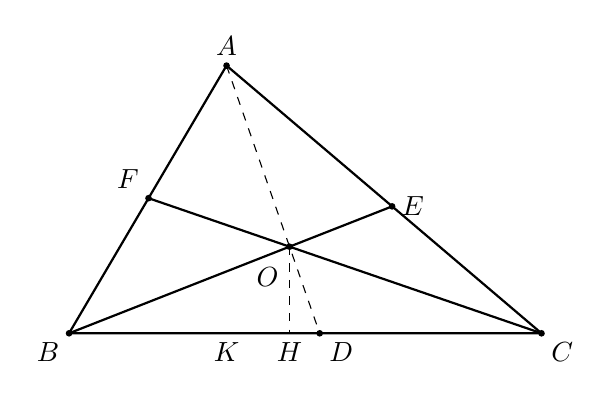
\begin{tikzpicture}[scale=1.0]
  \coordinate (A) at (2.0,3.4);
  \coordinate (B) at (0,0);
  \coordinate (C) at (6,0);
  \coordinate (O) at (2.8,1.1);
  \coordinate (D) at (3.183,0);
  \coordinate (E) at (4.103,1.612);
  \coordinate (F) at (1.009,1.716);
  \coordinate (K) at (2.0,0);
  \coordinate (H) at (2.8,0);
  \draw[thick] (A)--(B)--(C)--cycle;
  \draw[thick] (B)--(E);
  \draw[thick] (C)--(F);
  \draw[dashed] (A)--(D);
  \draw[dashed] (O)--(H);
  \fill (A) circle (1.2pt) node[above] {$A$};
  \fill (B) circle (1.2pt) node[below left] {$B$};
  \fill (C) circle (1.2pt) node[below right] {$C$};
  \fill (O) circle (1.2pt);
  \fill (D) circle (1.2pt) node[below right] {$D$};
  \fill (E) circle (1.2pt) node[right] {$E$};
  \fill (F) circle (1.2pt) node[above left] {$F$};
  \node[below] at (K) {$K$};
  \node[below] at (H) {$H$};
  \node at (2.52,0.72) {$O$};
\end{tikzpicture}
\end{center}
\nopagebreak[4]
\end{question}
\begin{question}
\gkti{7}\textbf{（12 分）} 设 $x$、$y$、$z$ 为三个互不相等的实数，且

\nopagebreak[4]
\[
x+\frac1y=y+\frac1z=z+\frac1x,
\]

求证：$x^2y^2z^2=1$。

\begin{gktip}
\textbf{参考题}（不计分，可以不做）
\end{gktip}

\textbf{参考题 1．} 将抛物线 $y=x^2$，直线 $x=2$ 与 $x$ 轴围成的曲边三角形，绕 $x$ 轴旋转一周形成一个旋转体，求此旋转体的体积。

\Needspace{5\baselineskip}
\textbf{参考题 2．} 求不定积分

\nopagebreak[4]
\[
\int\frac{6x^2+22x+18}{(x+1)(x+2)(x+3)}\,\mathrm dx.
\]

\end{question}